\documentclass[12pt,a4paper]{report}

% =========================================================================
% GOI THU VIEN VA CAU HINH CO BAN
% =========================================================================
\usepackage{fontspec}
\setmainfont{Times New Roman}

\usepackage[top=2.5cm,bottom=2.5cm,left=3.0cm,right=2.0cm]{geometry}
\usepackage{amsmath,amsfonts,amssymb}
\usepackage{graphicx}
\usepackage{booktabs}
\usepackage{tabularx}
\usepackage{multirow}
\usepackage{array}
\usepackage{float}
\usepackage{xcolor}
\usepackage{tikz}
\usetikzlibrary{calc,positioning,shapes.geometric,arrows.meta}
\usepackage{pgfornament}
\usepackage{setspace}
\usepackage{hyperref}
\usepackage{fancyhdr}
\usepackage{titlesec}
\usepackage{caption}
\usepackage{subcaption}
\usepackage{enumitem}
\usepackage{listings}

\graphicspath{{images/generated/}{images/}}
\renewcommand{\arraystretch}{1.12}
\renewcommand{\contentsname}{Mục lục}
\renewcommand{\listfigurename}{Danh mục hình ảnh}
\renewcommand{\listtablename}{Danh mục bảng biểu}
\renewcommand{\chaptername}{Chương}
\renewcommand{\figurename}{Hình}
\renewcommand{\tablename}{Bảng}
\renewcommand{\lstlistingname}{Đoạn mã}

% Toan bo chu va lien ket trong tai lieu duoc hien thi bang mau den.
\hypersetup{
    colorlinks=true,
    linkcolor=black,
    citecolor=black,
    urlcolor=black,
    pdftitle={Bao Cao Ky Thuat Assignment 04 - Convolutional Neural Networks},
    pdfauthor={Duong Trong Thang}
}

% Code listing don sac.
\lstdefinestyle{mystyle}{
    backgroundcolor=\color{white},
    commentstyle=\color{black},
    keywordstyle=\color{black}\bfseries,
    numberstyle=\tiny\color{black},
    stringstyle=\color{black},
    basicstyle=\ttfamily\footnotesize\color{black},
    breakatwhitespace=false,
    breaklines=true,
    captionpos=b,
    keepspaces=true,
    numbers=left,
    numbersep=5pt,
    showspaces=false,
    showstringspaces=false,
    showtabs=false,
    tabsize=2,
    frame=single,
    rulecolor=\color{black}
}
\lstset{style=mystyle}

% Dinh dang tieu de don sac.
\titleformat{\chapter}[display]
  {\normalfont\bfseries\color{black}}
  {\filleft\Large\bfseries\chaptertitlename\ \thechapter}
  {1ex}
  {\titlerule\vspace{1ex}\filright\LARGE}
  [\vspace{1ex}\titlerule]

\titleformat{\section}
  {\normalfont\Large\bfseries\color{black}}
  {\thesection}{1em}{}

\titleformat{\subsection}
  {\normalfont\large\bfseries\color{black}}
  {\thesubsection}{1em}{}

% Header va footer.
\pagestyle{fancy}
\fancyhf{}
\fancyhead[R]{\small\itshape Assignment 04: Convolutional Neural Networks}
\fancyfoot[C]{\thepage}
\renewcommand{\headrulewidth}{0.4pt}
\renewcommand{\footrulewidth}{0.4pt}
\setlength{\headheight}{14pt}

\newcommand{\modelpath}[1]{\texttt{#1}}
\newcommand{\best}[1]{\textbf{#1}}

% Khung trang bia theo mau duoc chon.
\newcommand{\decoratedframe}{%
  \begin{tikzpicture}[remember picture,overlay]
    \draw[line width=1.6pt]
      ($(current page.north west)+(1.2cm,-1.2cm)$) rectangle
      ($(current page.south east)+(-1.2cm,1.2cm)$);
    \draw[line width=0.8pt]
      ($(current page.north west)+(1.05cm,-1.05cm)$) rectangle
      ($(current page.south east)+(-1.05cm,1.05cm)$);
    \node[anchor=north west] at ($(current page.north west)+(1.18cm,-1.00cm)$)
      {\pgfornament[width=2.2cm]{61}};
    \node[anchor=north east] at ($(current page.north east)+(-1.18cm,-1.00cm)$)
      {\pgfornament[width=2.2cm,symmetry=v]{61}};
    \node[anchor=south west] at ($(current page.south west)+(1.18cm,1.00cm)$)
      {\pgfornament[width=2.2cm,symmetry=h]{61}};
    \node[anchor=south east] at ($(current page.south east)+(-1.18cm,1.00cm)$)
      {\pgfornament[width=2.2cm,symmetry=c]{61}};
  \end{tikzpicture}%
}

% Uu tien tep logo neu duoc bo sung; neu khong thi dung logo chu don sac.
\newcommand{\fallbacklogo}{%
  
\begin{tikzpicture}
    \node[
      text=black,
      font=\bfseries\fontsize{34}{38}\selectfont,
      inner sep=1pt
    ] (ptit) {PTIT};
    \node[
      star,
      star points=5,
      star point ratio=2.2,
      fill=black,
      draw=black,
      minimum size=0.78cm,
      inner sep=0pt
    ] at ($(ptit.north)+(0.20cm,-0.06cm)$) {};
    \draw[black,line width=1.1pt]
      ($(ptit.south west)+(-0.10cm,-0.18cm)$) --
      ($(ptit.south east)+(0.10cm,-0.18cm)$);
    \draw[black,line width=0.45pt]
      ($(ptit.south west)+(-0.10cm,-0.25cm)$) --
      ($(ptit.south east)+(0.10cm,-0.25cm)$);
  \end{tikzpicture}%
}

\newcommand{\showlogo}{%
  \begingroup
  \def\logoW{4cm}%
  \IfFileExists{photos/ptit.jpg}
    {
\includegraphics[width=\logoW]{photos/ptit.jpg}}{%
    \IfFileExists{photos/logo.png}
      {\includegraphics[width=\logoW]{photos/logo.png}}{%
      \IfFileExists{images/generated/ptit.jpg}
        {
\includegraphics[width=\logoW]{images/generated/ptit.jpg}}{%
        \fallbacklogo}}}%
  \endgroup
}

% =========================================================================
% BAT DAU TAI LIEU
% =========================================================================
\begin{document}
\color{black}

% -------------------------------------------------------------------------
% TRANG BIA
% -------------------------------------------------------------------------
\newgeometry{margin=2.2cm}
\hypersetup{pageanchor=false}
\begin{titlepage}
\setstretch{1.3}
\setlength{\parskip}{6pt}
\thispagestyle{empty}
\decoratedframe
\centering
\vspace*{1.2cm}

{\large\textbf{HỌC VIỆN CÔNG NGHỆ BƯU CHÍNH VIỄN THÔNG}}\\[4pt]
{\large\textbf{KHOA CÔNG NGHỆ THÔNG TIN 1}}\\[10pt]
\rule{7cm}{0.4pt}\\[0.8cm]

\showlogo\\[0.5cm]

{\huge\bfseries BÁO CÁO ASSIGNMENT 04}\\[10pt]
{\Large\bfseries MÔN HỌC: PHÁT TRIỂN HỆ THỐNG THÔNG MINH}\\[15pt]

{\textbf{Lớp D23CTPM01}}\\[6pt]
{\large\textbf{Giảng viên: Trần Đình Quế}}\\[0.8cm]

\begin{spacing}{1.2}
\setlength{\tabcolsep}{10pt}
\begin{tabular}{@{}>{\raggedright\arraybackslash}p{6.2cm} >{\raggedright\arraybackslash}p{4.2cm}@{}}
\textbf{Họ và Tên} & \textbf{Dương Trọng Thắng} \\
\textbf{Mã sinh viên} & \textbf{B23DCCN752} \\
\end{tabular}
\end{spacing}

\vfill
{\large\itshape Hà Nội -- 2026}
\end{titlepage}
\restoregeometry
\hypersetup{pageanchor=true}

% -------------------------------------------------------------------------
% MUC LUC VA DANH MUC
% -------------------------------------------------------------------------
\pagenumbering{roman}
\tableofcontents
\newpage
\listoffigures
\newpage
\listoftables
\newpage
\pagenumbering{arabic}

% -------------------------------------------------------------------------
% THONG TIN DU AN
% -------------------------------------------------------------------------
\chapter*{Thông tin dự án}
\addcontentsline{toc}{chapter}{Thông tin dự án}

\noindent\textbf{GitHub project:}
\url{https://github.com/duongthang2710/PTHTTM}

\vspace{0.35cm}
\noindent
Assignment 04 được tổ chức thành hai notebook độc lập cho MNIST và CIFAR-10.
Mỗi notebook thực hiện cùng một quy trình: tải dữ liệu, khảo sát phân phối lớp,
tách train/validation, chuẩn hóa, huấn luyện ba phiên bản CNN, đánh giá trên test
set và phân tích lỗi. Hai tệp nguồn dùng để đối chiếu toàn bộ số liệu trong báo
cáo là:
\begin{itemize}
    \item \modelpath{Assignment4/mnist/notebook/mnist\_cnn\_benchmark.ipynb};
    \item \modelpath{Assignment4/cifar10/notebook/cifar10\_cnn\_benchmark.ipynb}.
\end{itemize}

\noindent
Dữ liệu được notebook tải hoặc đọc từ thư mục \modelpath{data} cục bộ của từng
dataset. Các hình đã xuất từ output thực nghiệm nằm trong
\modelpath{Assignment4/Report/images/generated}; báo cáo \LaTeX{} nằm trong
\modelpath{Assignment4/Report}.
\newpage

% =========================================================================
% CHUONG 1
% =========================================================================
\chapter{Bài toán, dữ liệu và quy trình đánh giá}

\section{Mục tiêu và phạm vi thực nghiệm}
Assignment 04 khảo sát bài toán phân loại ảnh đa lớp bằng ba mức độ cài đặt:
\begin{enumerate}
    \item \textbf{CNN thuần NumPy}: tự hiện thực convolution, max pooling,
    dense, softmax--cross-entropy, backpropagation và Adam, không dùng autograd;
    \item \textbf{TensorFlow/Keras}: xây dựng mô hình bằng API cấp cao,
    automatic differentiation và pipeline \texttt{tf.data};
    \item \textbf{PyTorch}: định nghĩa module và training loop tường minh,
    đồng thời tận dụng backend tăng tốc của framework.
\end{enumerate}

Mục tiêu không chỉ là tìm accuracy cao nhất. Thực nghiệm còn ghi nhận
Macro-Precision, Macro-Recall, Macro-F1, số tham số, epoch tốt nhất, learning
rate cuối, thời gian huấn luyện và thời gian dự đoán. Cách thiết kế này cho phép
đối chiếu đồng thời chất lượng dự báo, độ phức tạp và mức độ thuận tiện của ba
cách cài đặt.

\section{Hai bộ dữ liệu ở hai mức độ khó}
\begin{table}[H]
\centering
\caption{Tổng quan dữ liệu dùng trong Assignment 04}
\label{tab:dataset_overview}
\resizebox{\textwidth}{!}{%
\begin{tabular}{llllll}
\toprule
\textbf{Dataset} & \textbf{Train gốc} & \textbf{Test} & \textbf{Kích thước ảnh} & \textbf{Số lớp} & \textbf{Đặc điểm} \\
\midrule
MNIST & 60,000 & 10,000 & $28\times28\times1$ & 10 & Chữ số viết tay, nền đơn giản \\
CIFAR-10 & 50,000 & 10,000 & $32\times32\times3$ & 10 & Vật thể tự nhiên, nền và góc nhìn đa dạng \\
\bottomrule
\end{tabular}%
}
\end{table}

MNIST gồm ảnh xám của mười chữ số viết tay. Đối tượng thường nằm gần trung tâm,
nền tối và hình dạng tương đối rõ nên bộ dữ liệu phù hợp để kiểm tra tính đúng
đắn của CNN tự cài đặt. CIFAR-10 gồm ảnh màu thuộc mười nhóm vật thể. Độ phân
giải chỉ $32\times32$ trong khi nền, góc nhìn, màu sắc và hình dạng thay đổi
mạnh, vì vậy mô hình cần học đặc trưng phức tạp hơn. Sự chênh lệch này giúp thể
hiện rõ giới hạn của CNN nông và lợi ích của residual learning.

\section{Tách dữ liệu và chuẩn hóa}
Notebook dùng \texttt{RANDOM\_STATE = 42} và tách train/validation theo nhãn
bằng \texttt{stratify}. Hai framework sử dụng toàn bộ phần train còn lại sau
khi giữ validation set; CNN NumPy dùng subset stratified để backpropagation thủ
công vẫn có thời gian chạy khả thi. Tất cả mô hình của cùng dataset được đánh
giá trên cùng full test set.

\begin{table}[H]
\centering
\caption{Kích thước các tập dữ liệu thực tế trong hai notebook}
\label{tab:data_splits}
\begin{tabular}{lrrrrr}
\toprule
\textbf{Dataset} & \textbf{Framework train} & \textbf{Validation} & \textbf{Test} & \textbf{NumPy train} & \textbf{NumPy val} \\
\midrule
MNIST & 54,000 & 6,000 & 10,000 & 20,000 & 3,000 \\
CIFAR-10 & 45,000 & 5,000 & 10,000 & 15,000 & 3,000 \\
\bottomrule
\end{tabular}
\end{table}

Ảnh được đổi sang \texttt{float32}, chia cho 255 rồi chuẩn hóa theo từng channel.
Mean và standard deviation chỉ được tính từ framework train set; cùng thống kê
đó sau đó được áp dụng cho validation, test và subset NumPy:
\begin{equation}
    \mathbf{X}_{norm}=
    \frac{\mathbf{X}/255-\boldsymbol{\mu}_{train}}
    {\boldsymbol{\sigma}_{train}+10^{-7}}.
\end{equation}
Quy trình này tránh dùng thông tin từ validation hoặc test trong tiền xử lý.
Test set cũng không tham gia chọn epoch, learning rate hay checkpoint.

\section{Metric và nguyên tắc đọc kết quả}
Accuracy đo tỉ lệ mẫu được phân loại đúng:
\begin{equation}
    \operatorname{Accuracy}=\frac{\text{số dự đoán đúng}}{N}.
\end{equation}
Với từng lớp $k$, precision, recall và F1 được tính theo one-vs-rest. Macro
average lấy trung bình không trọng số trên mười lớp, chẳng hạn:
\begin{equation}
    \operatorname{MacroF1}=\frac{1}{K}\sum_{k=1}^{K}F1_k.
\end{equation}
Macro-F1 giúp mỗi lớp có ảnh hưởng ngang nhau, đặc biệt hữu ích khi phân phối
MNIST không hoàn toàn đều. Trong notebook, bảng kết quả được sắp theo Macro-F1
rồi Accuracy. Ma trận nhầm lẫn chuẩn hóa và accuracy theo lớp được dùng để bổ
sung cho các score tổng hợp; nhóm ảnh dự đoán sai có confidence cao nhất giúp
kiểm tra kiểu lỗi cụ thể.

Thời gian huấn luyện và dự đoán chỉ phản ánh lần chạy đã lưu. NumPy dùng ít mẫu
hơn, kiến trúc khác framework và các framework chịu ảnh hưởng của backend,
compilation, warm-up cùng tải hệ thống. Vì vậy các số thời gian không được xem
như benchmark phần cứng tuyệt đối.

% =========================================================================
% CHUONG 2
% =========================================================================
\chapter{Từ nền tảng CNN đến ba cách cài đặt}

\section{Phép tích chập và feature map}
Ảnh số được biểu diễn bởi tensor
$\mathbf{X}\in\mathbb{R}^{H\times W\times C}$. Một CNN ánh xạ ảnh sang logits
$\mathbf{z}\in\mathbb{R}^{K}$, sau đó softmax chuyển logits thành phân phối xác
suất. So với việc làm phẳng ảnh ngay từ đầu, convolution giữ quan hệ lân cận,
dùng kết nối cục bộ và chia sẻ cùng kernel ở nhiều vị trí.

Với kernel $K_h\times K_w$, stride $S$ và padding $P$, feature map thứ $k$ có
phần tử:
\begin{equation}
Y_{i,j,k}=b_k+
\sum_{u=0}^{K_h-1}
\sum_{v=0}^{K_w-1}
\sum_{c=0}^{C-1}
X_{iS+u-P,\,jS+v-P,\,c}W_{u,v,c,k}.
\end{equation}
Kích thước không gian đầu ra là:
\begin{align}
H_{out} &= \left\lfloor\frac{H+2P-K_h}{S}\right\rfloor+1,\\
W_{out} &= \left\lfloor\frac{W+2P-K_w}{S}\right\rfloor+1.
\end{align}
Các convolution trong notebook dùng kernel $3\times3$. Với padding 1 và stride
1, chiều cao và chiều rộng được giữ nguyên.

\section{ReLU, pooling và receptive field}
Sau convolution, ReLU tạo tính phi tuyến:
\begin{equation}
    \operatorname{ReLU}(z)=\max(0,z).
\end{equation}
Max pooling $2\times2$ lấy kích hoạt lớn nhất trong từng vùng và giảm một nửa
kích thước không gian. Việc xếp chồng nhiều convolution làm receptive field
tăng dần, cho phép neuron ở tầng sâu tổng hợp thông tin từ vùng lớn hơn của ảnh.

CNN NumPy trong cả hai notebook có pipeline:
\begin{equation}
\text{Conv--ReLU--Pool}
\to\text{Conv--ReLU--Pool}
\to\text{Dense--ReLU}
\to\text{Dense}.
\end{equation}
Kiến trúc đủ ngắn để tự hiện thực toàn bộ forward/backward nhưng vẫn tạo hai cấp
feature map.

\section{Softmax, Cross-Entropy và backpropagation}
Với logits $\mathbf{z}$, xác suất của lớp $k$ là:
\begin{equation}
    \hat{y}_k=\frac{\exp(z_k-\max_j z_j)}
    {\sum_{r=1}^{K}\exp(z_r-\max_j z_j)}.
\end{equation}
Phép trừ logits lớn nhất trước khi lấy hàm mũ giúp tránh overflow. Loss trung
bình trên mini-batch $m$ mẫu được tính bởi:
\begin{equation}
    \mathcal{L}_{CE}=-\frac{1}{m}\sum_{i=1}^{m}
    \log\!\left(\hat{y}_{i,y_i}\right).
\end{equation}
Đúng với hàm \texttt{SoftmaxCrossEntropy.backward} trong notebook, gradient theo
logits là:
\begin{equation}
    \frac{\partial\mathcal{L}}{\partial\mathbf{z}_i}
    =\frac{\hat{\mathbf{y}}_i-\mathbf{y}_i}{m}.
\end{equation}

Trong convolution, gradient trọng số được cộng dồn từ mọi vị trí sử dụng cùng
kernel. CNN NumPy trích các cửa sổ bằng
\texttt{sliding\_window\_view} và dùng \texttt{einsum} cho phép nhân tensor.
Max pooling lưu mask cực đại; nếu một vùng có nhiều giá trị cực đại bằng nhau,
gradient được chia đều cho các vị trí đó. Các lớp dense áp dụng:
\begin{align}
    \frac{\partial\mathcal{L}}{\partial\mathbf{W}}
    &=\mathbf{A}^{\top}\frac{\partial\mathcal{L}}{\partial\mathbf{Z}},\\
    \frac{\partial\mathcal{L}}{\partial\mathbf{b}}
    &=\sum_i\frac{\partial\mathcal{L}}{\partial\mathbf{Z}_i},\\
    \frac{\partial\mathcal{L}}{\partial\mathbf{A}}
    &=\frac{\partial\mathcal{L}}{\partial\mathbf{Z}}\mathbf{W}^{\top}.
\end{align}

\section{Training loop thuần NumPy}
Mỗi epoch hoán vị train set, tăng cường từng mini-batch, thực hiện forward,
backward và cập nhật Adam. Gradient của từng tensor được clip theo phần tử trong
$[-5,5]$; weight decay chỉ áp dụng cho ma trận trọng số. Learning rate giảm theo
cosine từ $10^{-3}$ xuống $5\times10^{-5}$.

\begin{lstlisting}[language=Python,caption={Luồng huấn luyện CNN NumPy trong notebook},label={lst:numpy_training}]
for epoch in range(epochs):
    lr = cosine_learning_rate(initial_lr, epoch, epochs)
    indices = rng.permutation(len(X_train))

    for start in range(0, len(indices), batch_size):
        batch_ids = indices[start:start + batch_size]
        X_batch = augment_numpy_batch(X_train[batch_ids], rng, dataset_key)
        y_batch = y_train[batch_ids]

        logits = model.forward(X_batch)
        loss = criterion.forward(logits, y_batch)
        model.backward(criterion.backward())
        optimizer.step(model.named_parameters(), learning_rate=lr)

    if validation_loss < best_loss:
        best_state = model.state_dict()

model.load_state_dict(best_state)
\end{lstlisting}

Optimizer chỉ nhận gradient từ train loss. Cuối mỗi epoch, validation loss và
validation accuracy được tính độc lập. CNN NumPy lưu checkpoint có validation
loss thấp nhất; Keras và PyTorch lưu checkpoint có validation accuracy cao nhất.
Trạng thái tốt nhất được khôi phục trước khi dự đoán test set.

\section{Cấu hình mô hình và chính sách huấn luyện}
\begin{table}[H]
\centering
\caption{Cấu hình CNN NumPy theo từng dataset}
\label{tab:numpy_config}
\resizebox{\textwidth}{!}{%
\begin{tabular}{lcccccccc}
\toprule
\textbf{Dataset} & \textbf{Filters} & \textbf{Hidden} & \textbf{Epoch} & \textbf{Batch} & \textbf{LR đầu} & \textbf{Weight decay} & \textbf{Tham số} & \textbf{Augmentation} \\
\midrule
MNIST & $(8,16)$ & 64 & 15 & 64 & $10^{-3}$ & $10^{-4}$ & 52,138 & Dịch tối đa 2 px \\
CIFAR-10 & $(12,24)$ & 128 & 50 & 64 & $10^{-3}$ & $10^{-4}$ & 200,978 & Crop 4 px, flip \\
\bottomrule
\end{tabular}%
}
\end{table}

\begin{table}[H]
\centering
\caption{Kiến trúc và cấu hình hai framework}
\label{tab:framework_config}
\resizebox{\textwidth}{!}{%
\begin{tabular}{lllll}
\toprule
\textbf{Dataset} & \textbf{Kiến trúc} & \textbf{Optimizer} & \textbf{Epoch / Batch} & \textbf{Regularization} \\
\midrule
MNIST & 2 block Conv-BN-ReLU-Pool, Dense 128 & AdamW, LR $10^{-3}$ & 15 / 128 & Dropout 0.15, 0.25, 0.30 \\
CIFAR-10 & ResNet-20, stage $16\to32\to64$ & SGD, momentum 0.9, Nesterov & 50 / 256 & L2 $5\times10^{-4}$, smoothing 0.1 \\
\bottomrule
\end{tabular}%
}
\end{table}

Trên MNIST, Keras và PyTorch có cùng topology trainable: mỗi block chứa hai
convolution $3\times3$, Batch Normalization và ReLU, tiếp theo là max pooling và
Dropout; phần phân loại dùng Dense 128 rồi output 10 lớp. Hai framework dùng
AdamW và giảm learning rate khi validation accuracy ngừng cải thiện.

Trên CIFAR-10, hai framework dùng ResNet-20: stem 16 channel, ba stage
$16\to32\to64$, mỗi stage có ba residual block, sau cùng là Global Average
Pooling và lớp tuyến tính 10 đầu ra. Khi kích thước hoặc số channel thay đổi,
nhánh tắt dùng convolution $1\times1$ với stride tương ứng. Cả hai dùng SGD,
momentum 0.9, Nesterov, warm-up 5 epoch từ 0.02 lên 0.10 và cosine decay;
Cross-Entropy có label smoothing 0.1.

Augmentation chỉ áp dụng cho train. MNIST dùng reflect padding/crop hoặc phép
tịnh tiến tương đương với độ dịch tối đa 2 pixel. CIFAR-10 dùng dịch tối đa 4
pixel và horizontal flip với xác suất 0.5. Validation và test không augmentation.

\section{Vị trí của residual network trong tiến trình CNN}
\begin{table}[H]
\centering
\caption{Một số hướng phát triển tiêu biểu từ CNN cơ bản}
\label{tab:cnn_evolution}
\resizebox{\textwidth}{!}{%
\begin{tabular}{lll}
\toprule
\textbf{Kiến trúc} & \textbf{Cải tiến chính} & \textbf{Ý nghĩa} \\
\midrule
LeNet-5 & Conv, pooling và fully connected theo chuỗi & Nền tảng cho nhận dạng chữ số \\
AlexNet & ReLU, dropout, augmentation, GPU & Mở rộng CNN sâu lên ImageNet \\
VGG & Xếp chồng convolution $3\times3$ & Thiết kế đồng nhất nhưng nhiều tham số \\
Inception & Nhiều nhánh kernel và convolution $1\times1$ & Học đặc trưng đa tỉ lệ \\
ResNet & Skip/residual connection & Cải thiện luồng gradient trong mạng sâu \\
DenseNet & Nối feature từ các tầng trước & Tái sử dụng feature \\
MobileNet & Depthwise-separable convolution & Giảm FLOPs và số tham số \\
EfficientNet & Scale depth, width và resolution & Cân bằng chất lượng với chi phí \\
\bottomrule
\end{tabular}%
}
\end{table}

Residual block học $F(\mathbf{x})$ rồi cộng lại đầu vào,
$\mathbf{y}=F(\mathbf{x};\theta)+\mathbf{x}$. Đường truyền tắt giúp gradient đi
qua mạng sâu thuận lợi hơn. Đây là lý do ResNet-20 được chọn cho CIFAR-10, trong
khi mô hình nông vẫn đủ phù hợp với MNIST.

% =========================================================================
% CHUONG 3
% =========================================================================
\chapter{Đối chuẩn trên MNIST}

\section{Dữ liệu và cấu hình riêng}
MNIST có 60,000 ảnh train gốc và 10,000 ảnh test; pixel nằm trong khoảng 0 đến
255. Phân phối lớp không mất cân bằng nghiêm trọng nhưng không hoàn toàn đều:
lớp 1 có 6,742 ảnh train, còn lớp 5 có 5,421 ảnh.

\begin{figure}[H]
    \centering
    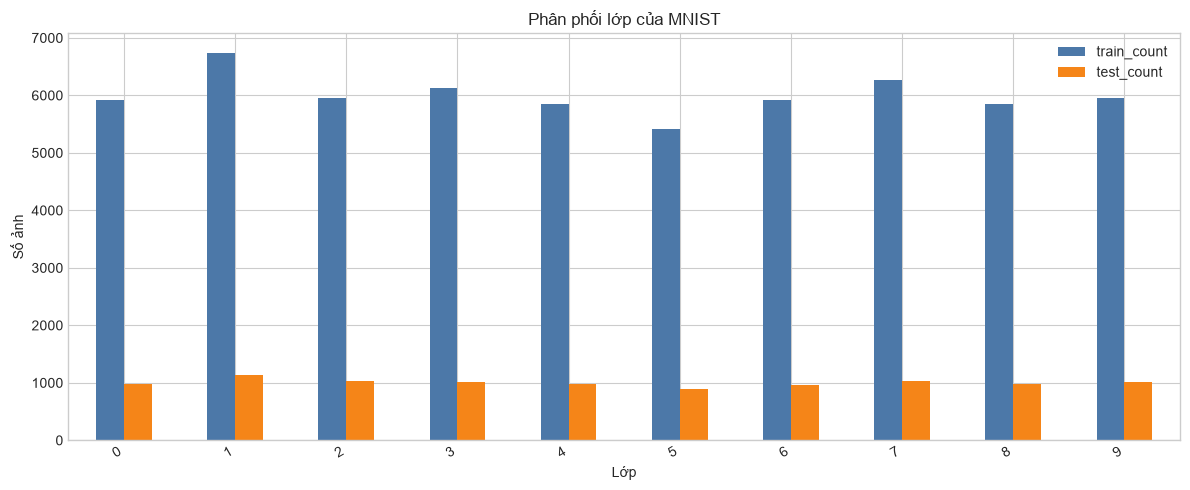
\includegraphics[width=0.95\textwidth]{mnist_class_distribution.png}
    \caption{Phân phối lớp của MNIST trên tập train gốc và test}
    \label{fig:mnist_distribution}
\end{figure}

\begin{figure}[H]
    \centering
    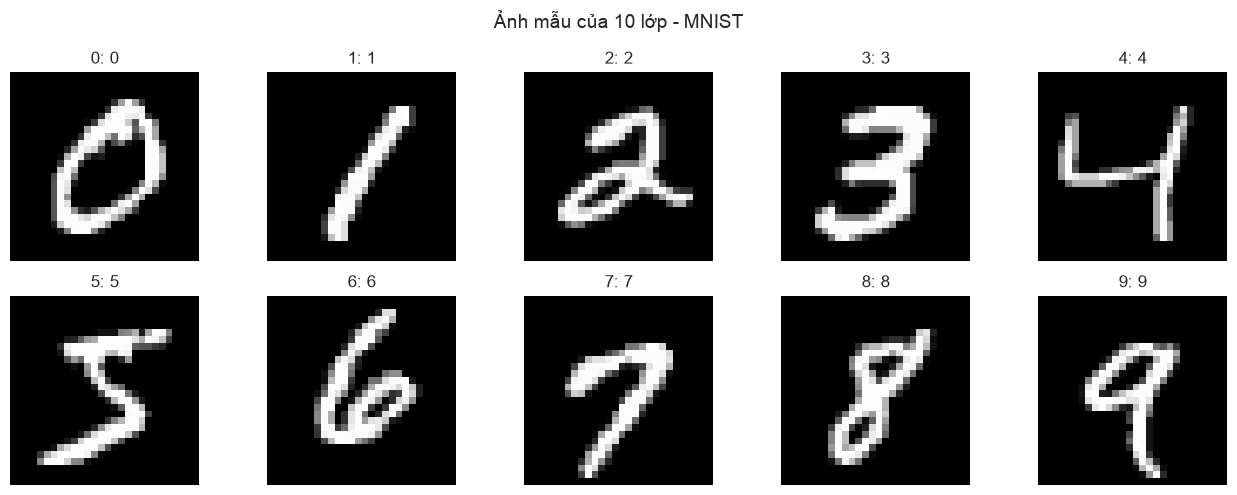
\includegraphics[width=\textwidth]{mnist_sample_images.png}
    \caption{Một ảnh đại diện cho mỗi lớp chữ số trong MNIST}
    \label{fig:mnist_samples}
\end{figure}

Framework train có 54,000 mẫu, validation có 6,000 mẫu; subset NumPy gồm 20,000
mẫu train và 3,000 mẫu validation. Thống kê chỉ học từ framework train là
$\mu=0.13073687$ và $\sigma=0.30819046$.

CNN NumPy có luồng kích thước
$28\times28\times1\to\text{Conv}(8)\to\text{Pool}
\to\text{Conv}(16)\to\text{Pool}\to\text{Dense}(64)\to10$,
với 52,138 tham số. Keras báo cáo 468,394 tham số tổng, gồm 468,010 tham số
trainable và 384 trạng thái không trainable của Batch Normalization. PyTorch có
468,010 tham số.

\section{Kết quả test set}
\begin{table}[H]
\centering
\caption{Benchmark ba cách cài đặt CNN trên MNIST}
\label{tab:mnist_benchmark}
\resizebox{\textwidth}{!}{%
\begin{tabular}{lcccccccccc}
\toprule
\textbf{Mô hình} & \textbf{Acc.} & \textbf{Macro-P} & \textbf{Macro-R} & \textbf{Macro-F1} & \textbf{Train} & \textbf{Epoch} & \textbf{LR cuối} & \textbf{Tham số} & \textbf{Train(s)} & \textbf{Pred(s)} \\
\midrule
PyTorch CNN & \best{0.9958} & \best{0.9959} & \best{0.9958} & \best{0.9958} & 54,000 & 14 & $3.0\!\times\!10^{-4}$ & 468,010 & 90.38 & \best{0.307} \\
TensorFlow/Keras CNN & 0.9955 & 0.9955 & 0.9955 & 0.9955 & 54,000 & 13 & $2.7\!\times\!10^{-5}$ & 468,394 & 399.87 & 1.183 \\
NumPy CNN from scratch & 0.9848 & 0.9847 & 0.9847 & 0.9847 & 20,000 & 13 & $5.0\!\times\!10^{-5}$ & \best{52,138} & \best{82.86} & 1.094 \\
\bottomrule
\end{tabular}%
}
\end{table}

PyTorch có Macro-F1 cao nhất 0.9958, hơn Keras 0.0003; chênh lệch về chất
lượng dự báo là rất nhỏ. Trong lần chạy lưu trong notebook, PyTorch dự đoán
nhanh nhất và train trong 90.38 giây trên MPS. CNN NumPy đạt accuracy 0.9848 dù
chỉ dùng 20,000 mẫu train và 52,138 tham số, cho thấy forward/backward thủ công
hoạt động đúng. Khoảng cách xấp xỉ 1.1 điểm phần trăm so với framework còn chịu
ảnh hưởng của lượng dữ liệu, độ lớn mô hình và primitive tối ưu mức thấp.

\begin{figure}[H]
    \centering
    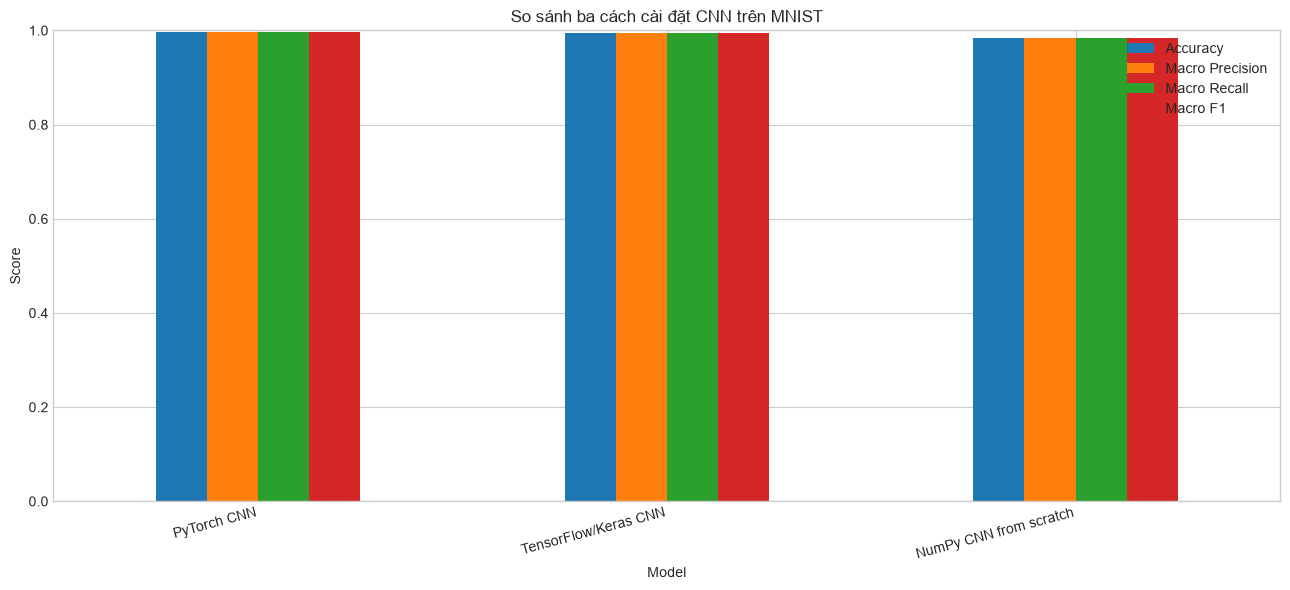
\includegraphics[width=\textwidth]{mnist_metric_comparison.png}
    \caption{Bốn metric phân loại của ba mô hình trên MNIST}
    \label{fig:mnist_metric_comparison}
\end{figure}

\section{Diễn biến huấn luyện}
\begin{figure}[H]
    \centering
    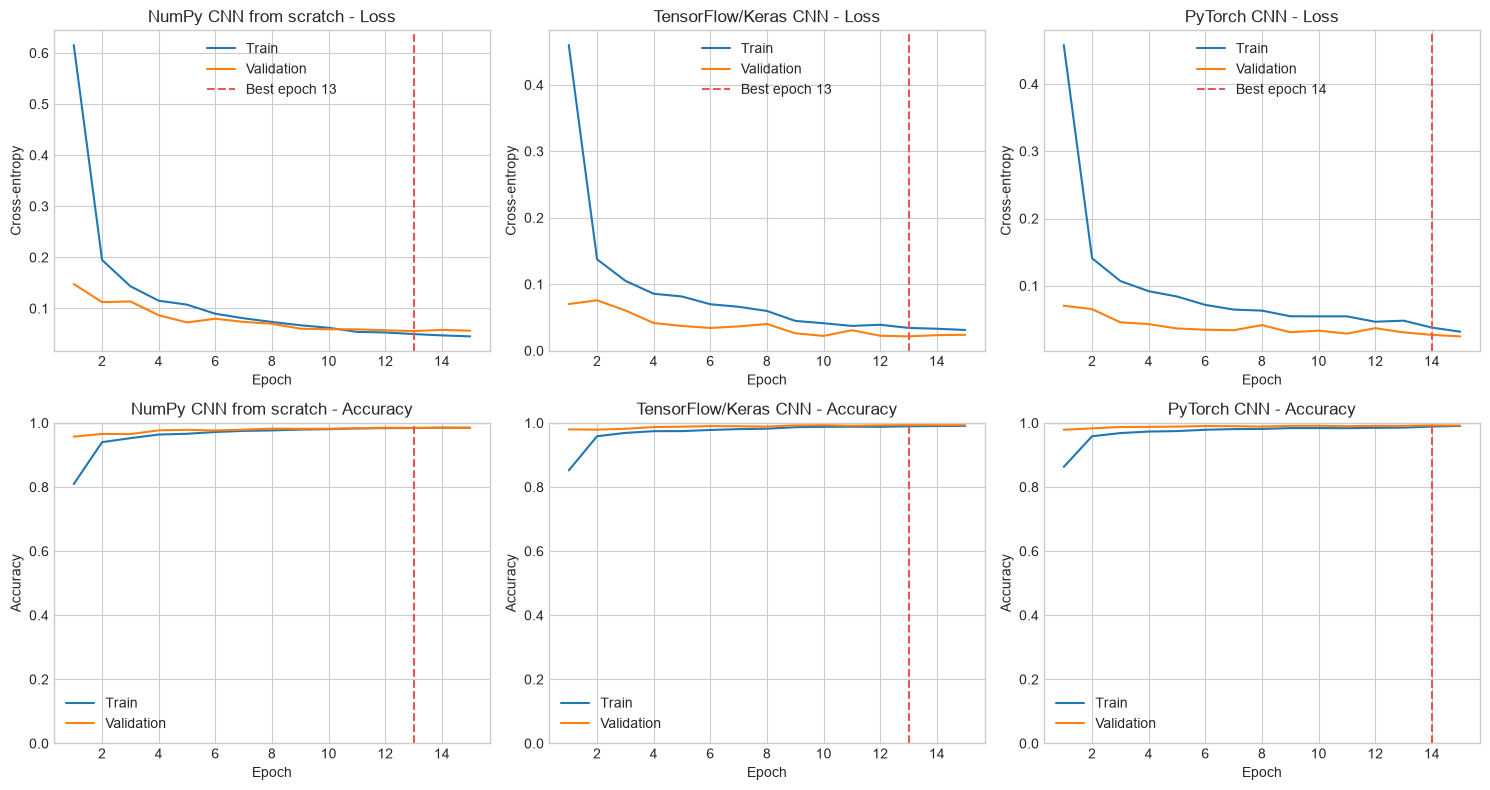
\includegraphics[width=\textwidth]{mnist_learning_curves.png}
    \caption{Train/validation loss và accuracy trên MNIST}
    \label{fig:mnist_learning_curves}
\end{figure}

CNN NumPy giảm validation loss từ 0.1477 ở epoch 1 xuống 0.0558 ở epoch 13.
Hai epoch sau có validation loss lần lượt 0.0581 và 0.0564, nên notebook khôi
phục checkpoint epoch 13. Keras đạt validation accuracy tốt nhất 0.9937 ở epoch
13; PyTorch đạt 0.9928 ở epoch 14. Các đường train/validation của framework hội
tụ trên 0.99 và không tách xa, cho thấy augmentation cùng regularization kiểm
soát overfitting tốt trong cấu hình này.

\section{Ma trận nhầm lẫn và phân tích lỗi}
\begin{figure}[H]
    \centering
    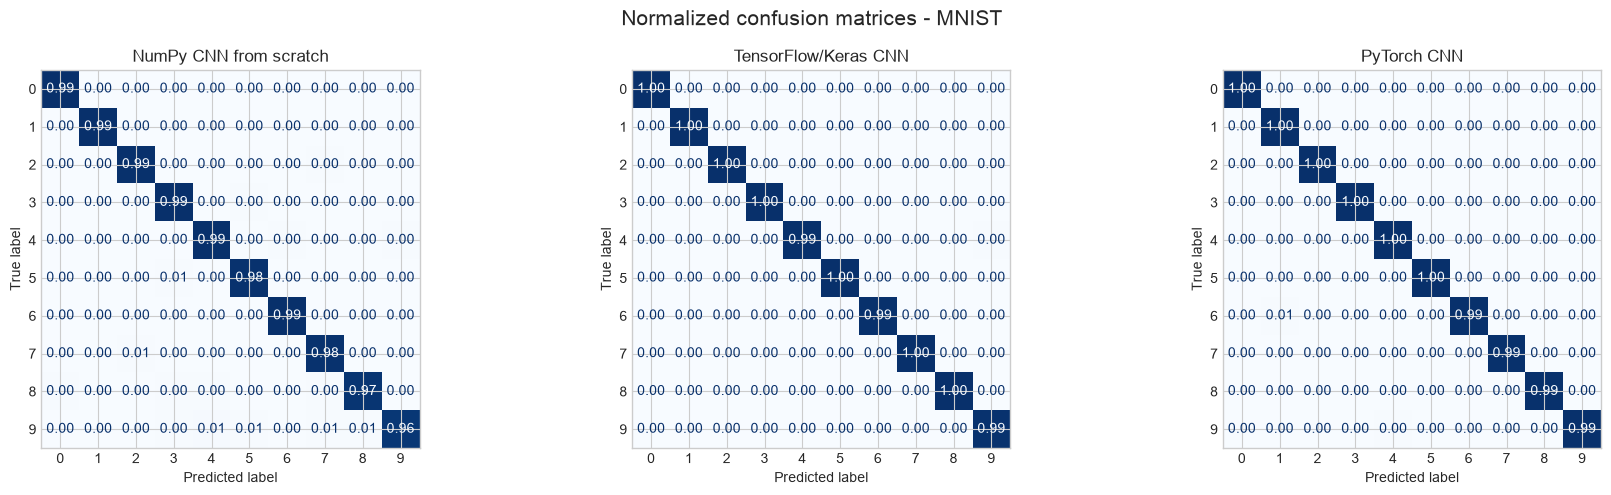
\includegraphics[width=\textwidth]{mnist_normalized_confusion_matrices.png}
    \caption{Ma trận nhầm lẫn chuẩn hóa của ba mô hình trên MNIST}
    \label{fig:mnist_confusion}
\end{figure}

Hai framework có ma trận gần như tập trung hoàn toàn trên đường chéo. CNN NumPy
yếu hơn ở chữ số 8 và 9, với recall hiển thị xấp xỉ 0.97 và 0.96. Các chữ số có
nét vòng hoặc nét kéo dài dễ bị nhầm khi cách viết không điển hình.

\begin{table}[H]
\centering
\caption{Accuracy theo lớp của mô hình tốt nhất trên MNIST (PyTorch CNN)}
\label{tab:mnist_per_class}
\begin{tabular}{crr@{\qquad}crr}
\toprule
\textbf{Lớp} & \textbf{Số mẫu} & \textbf{Accuracy} & \textbf{Lớp} & \textbf{Số mẫu} & \textbf{Accuracy} \\
\midrule
0 & 980 & 0.9990 & 5 & 892 & 0.9955 \\
1 & 1,135 & 0.9974 & 6 & 958 & 0.9927 \\
2 & 1,032 & 0.9971 & 7 & 1,028 & 0.9942 \\
3 & 1,010 & 0.9960 & 8 & 974 & 0.9949 \\
4 & 982 & 0.9990 & 9 & 1,009 & 0.9921 \\
\bottomrule
\end{tabular}
\end{table}

Lớp 0 và 4 cùng đạt 0.9990; lớp 9 thấp nhất nhưng vẫn đạt 0.9921. Notebook chọn
12 dự đoán sai có confidence lớn nhất của mô hình đứng đầu theo Macro-F1.

\begin{figure}[H]
    \centering
    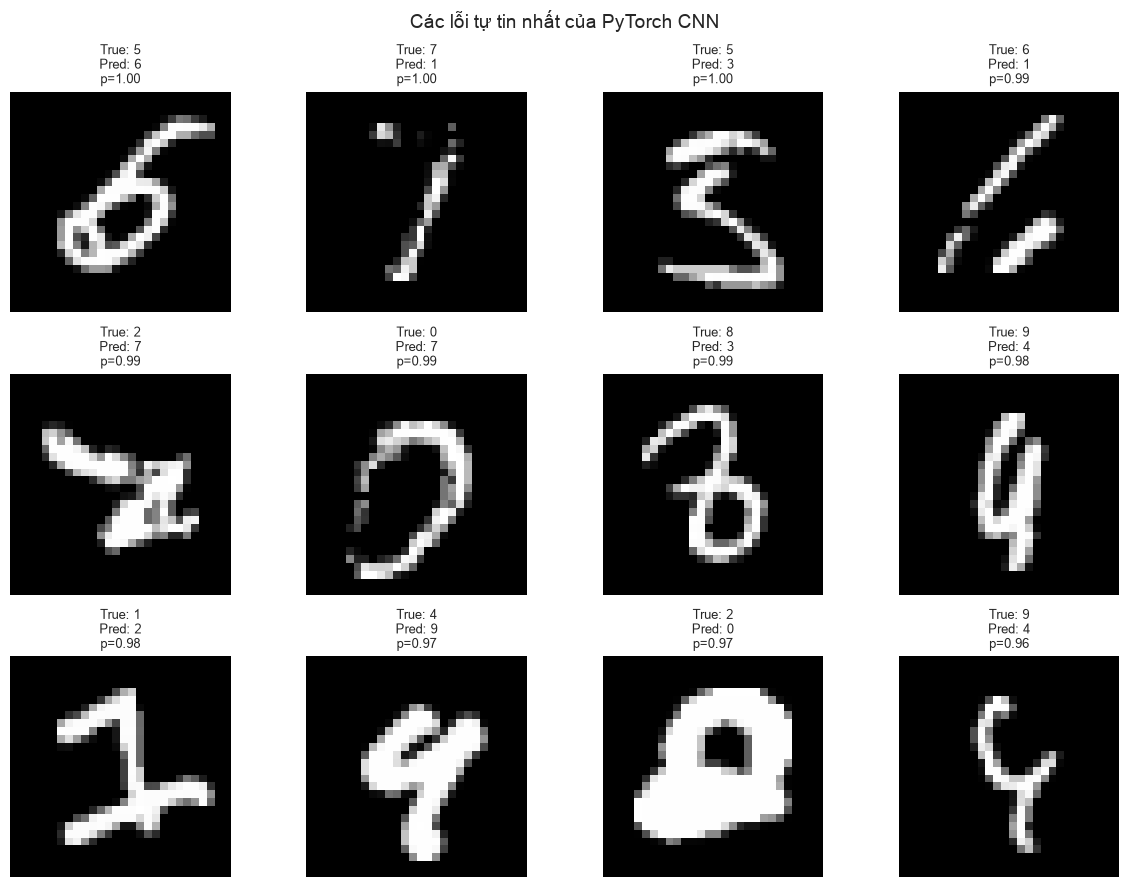
\includegraphics[width=0.88\textwidth]{mnist_prediction_error_analysis.png}
    \caption{Các lỗi có confidence cao nhất của PyTorch CNN trên MNIST}
    \label{fig:mnist_errors}
\end{figure}

Nhiều ảnh sai có nét viết mơ hồ: chữ số 5 gần giống 6 hoặc 3, chữ số 7 giống 1,
và chữ số 9 gần giống 4. Kết quả nhắc lại rằng confidence softmax cao không bảo
đảm dự đoán đúng khi hình dạng nằm ngoài kiểu phổ biến của train set.

% =========================================================================
% CHUONG 4
% =========================================================================
\chapter{Đối chuẩn trên CIFAR-10}

\section{Dữ liệu và cấu hình riêng}
CIFAR-10 có 50,000 ảnh train và 10,000 ảnh test thuộc các lớp
\textit{airplane, automobile, bird, cat, deer, dog, frog, horse, ship, truck}.
Mỗi lớp có đúng 5,000 ảnh train gốc và 1,000 ảnh test; vì test set cân bằng,
Accuracy và Macro-Recall bằng nhau trong bảng kết quả.

\begin{figure}[H]
    \centering
    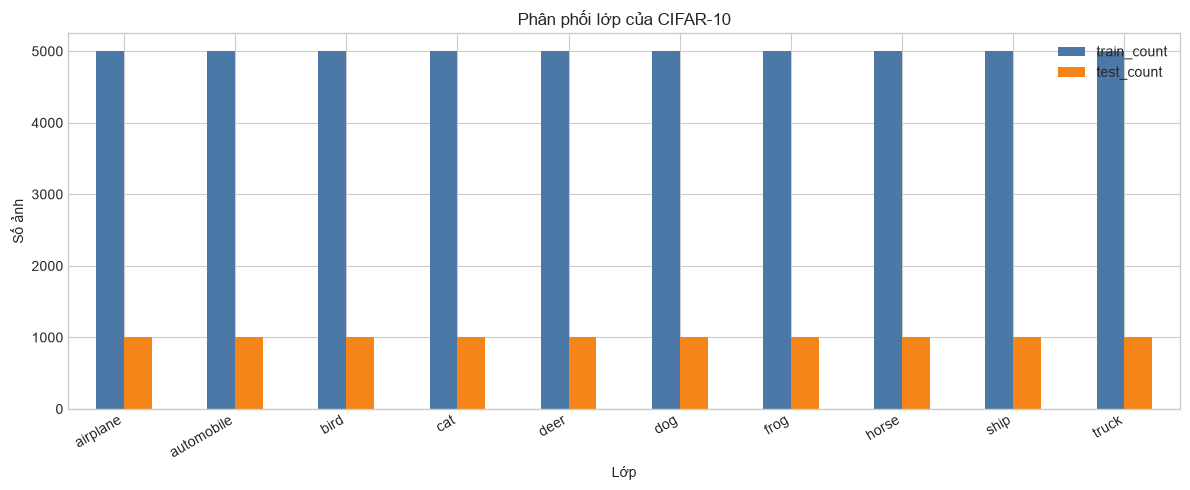
\includegraphics[width=0.95\textwidth]{cifar10_class_distribution.png}
    \caption{Phân phối cân bằng của CIFAR-10}
    \label{fig:cifar_distribution}
\end{figure}

\begin{figure}[H]
    \centering
    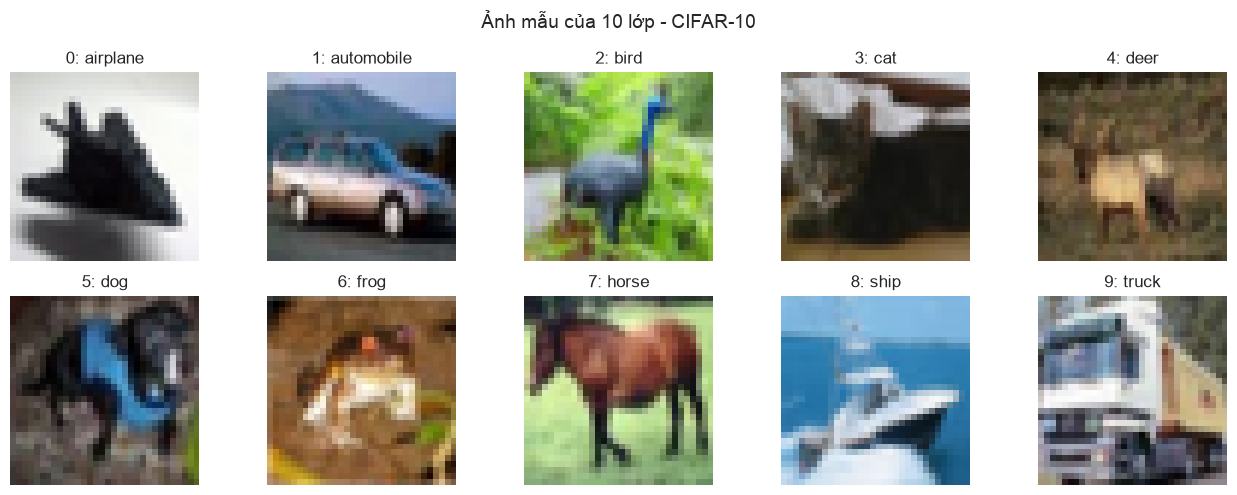
\includegraphics[width=\textwidth]{cifar10_sample_images.png}
    \caption{Một ảnh đại diện cho mỗi lớp trong CIFAR-10}
    \label{fig:cifar_samples}
\end{figure}

Framework train gồm 45,000 mẫu, validation gồm 5,000 mẫu. Subset NumPy có
15,000 mẫu train và 3,000 mẫu validation; riêng train subset có đúng 1,500 mẫu
mỗi lớp. Mean và standard deviation học từ framework train là:
\begin{align}
    \boldsymbol{\mu}_{train}
    &= (0.49113446,\ 0.48211210,\ 0.44644734),\\
    \boldsymbol{\sigma}_{train}
    &= (0.24686947,\ 0.24343061,\ 0.26160370).
\end{align}

CNN NumPy dùng 12 và 24 filter, hidden layer 128, tổng 200,978 tham số. Keras
ResNet-20 có 274,042 tham số tổng, gồm 272,474 trainable và 1,568 trạng thái
Batch Normalization; PyTorch ResNet-20 có 272,474 tham số.

\section{Kết quả test set}
\begin{table}[H]
\centering
\caption{Benchmark ba cách cài đặt CNN trên CIFAR-10}
\label{tab:cifar_benchmark}
\resizebox{\textwidth}{!}{%
\begin{tabular}{lcccccccccc}
\toprule
\textbf{Mô hình} & \textbf{Acc.} & \textbf{Macro-P} & \textbf{Macro-R} & \textbf{Macro-F1} & \textbf{Train} & \textbf{Epoch} & \textbf{LR cuối} & \textbf{Tham số} & \textbf{Train(s)} & \textbf{Pred(s)} \\
\midrule
PyTorch CNN & \best{0.9095} & \best{0.9092} & \best{0.9095} & \best{0.9092} & 45,000 & 48 & $2.22\!\times\!10^{-4}$ & 272,474 & 822.82 & \best{1.248} \\
TensorFlow/Keras CNN & 0.9078 & 0.9077 & 0.9078 & 0.9075 & 45,000 & 49 & $2.22\!\times\!10^{-4}$ & 274,042 & 2,636.45 & 4.125 \\
NumPy CNN from scratch & 0.7012 & 0.6987 & 0.7012 & 0.6994 & 15,000 & 47 & $5.0\!\times\!10^{-5}$ & \best{200,978} & \best{501.36} & 3.875 \\
\bottomrule
\end{tabular}%
}
\end{table}

PyTorch có Macro-F1 cao nhất 0.9092, hơn Keras 0.0017. Hai ResNet-20 gần
tương đương về chất lượng, nhưng thời gian của lần chạy đã lưu khác đáng kể:
822.82 giây so với 2,636.45 giây khi train và 1.248 giây so với 4.125 giây khi
dự đoán. Đây là kết quả theo backend MPS và môi trường cụ thể, không phải kết
luận rằng một framework luôn nhanh hơn framework còn lại.

CNN NumPy đạt accuracy 0.7012 và Macro-F1 0.6994. So với ResNet-20, khoảng cách
lớn phản ánh đồng thời kiến trúc nông, subset chỉ 15,000 ảnh, ít tham số hơn và
không có Batch Normalization hay residual connection.

\begin{figure}[H]
    \centering
    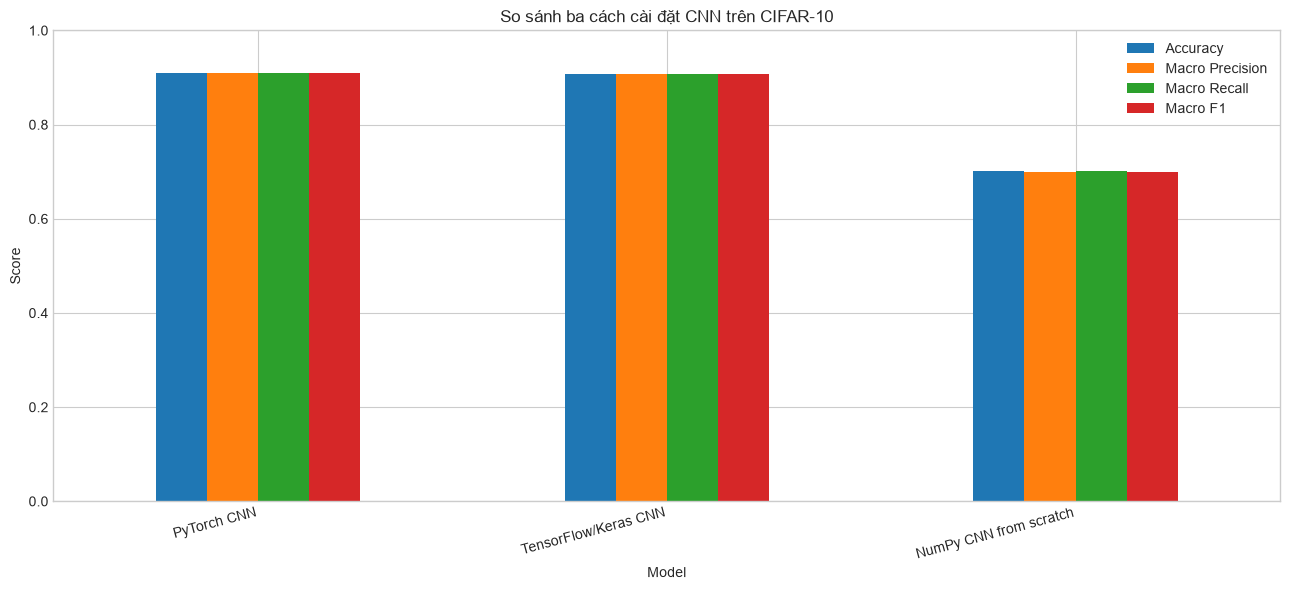
\includegraphics[width=\textwidth]{cifar10_metric_comparison.png}
    \caption{Bốn metric phân loại của ba mô hình trên CIFAR-10}
    \label{fig:cifar_metric_comparison}
\end{figure}

\section{Diễn biến huấn luyện}
\begin{figure}[H]
    \centering
    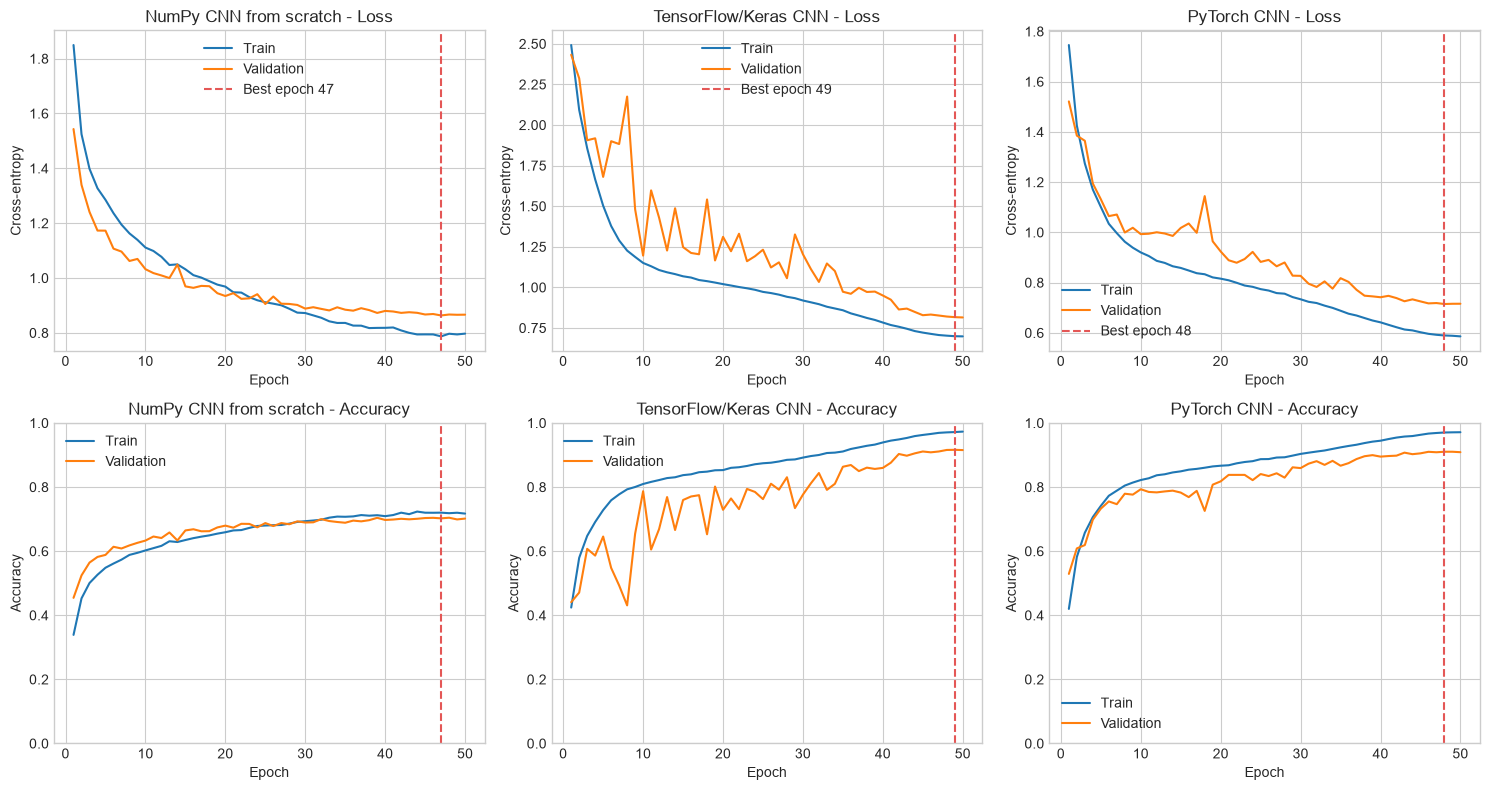
\includegraphics[width=\textwidth]{cifar10_learning_curves.png}
    \caption{Train/validation loss và accuracy trên CIFAR-10}
    \label{fig:cifar_learning_curves}
\end{figure}

CNN NumPy dừng quanh train/validation accuracy 0.72/0.70; validation loss tốt
nhất là 0.8634 tại epoch 47. Hai đường gần nhau cho thấy hạn chế chính là
underfitting hơn là overfitting.

Keras đạt validation accuracy tốt nhất 0.9162 ở epoch 49; PyTorch đạt 0.9102 ở
epoch 48. Keras có validation score cao hơn nhưng PyTorch nhỉnh hơn trên test,
cho thấy chênh lệch nhỏ có thể thay đổi theo split và trạng thái huấn luyện.
Validation metric dao động trong nửa đầu do augmentation, SGD và learning rate
lớn; khi cosine decay hạ learning rate về cuối, các đường cong ổn định hơn.

\section{Độ khó theo lớp và các lỗi nổi bật}
\begin{figure}[H]
    \centering
    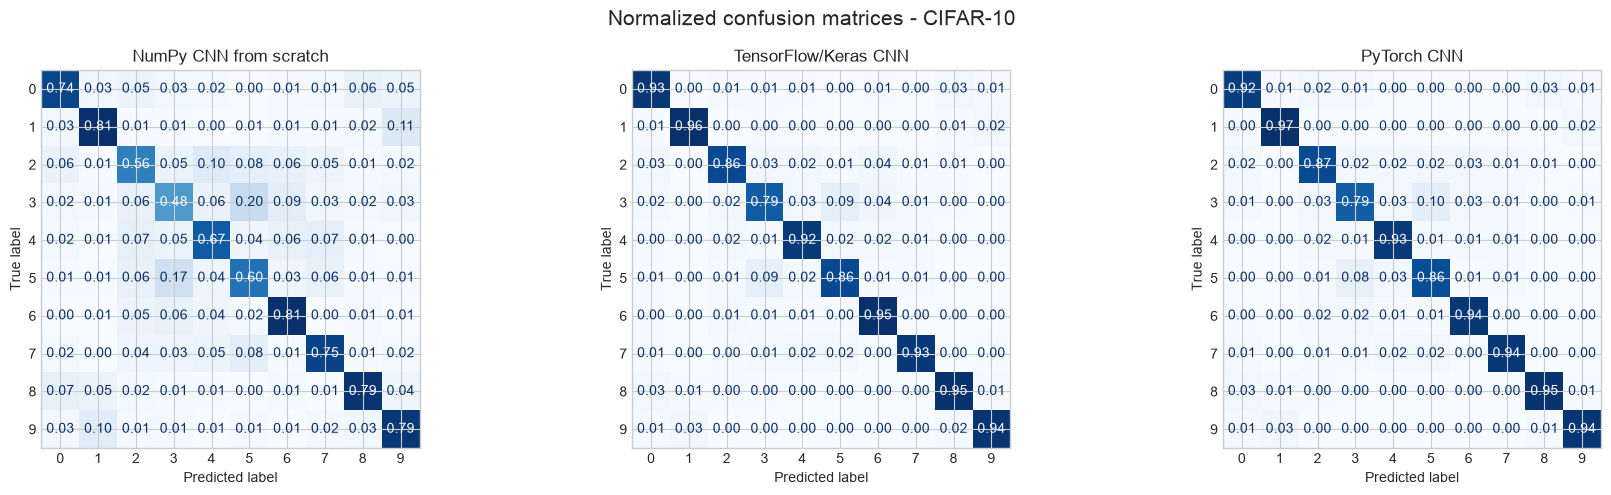
\includegraphics[width=\textwidth]{cifar10_normalized_confusion_matrices.png}
    \caption{Ma trận nhầm lẫn chuẩn hóa của ba mô hình trên CIFAR-10}
    \label{fig:cifar_confusion}
\end{figure}

CNN NumPy nhầm nhiều giữa các lớp động vật. Trong ma trận làm tròn, recall lớp
\textit{cat} chỉ khoảng 0.48 và khoảng 20\% ảnh mèo bị dự đoán thành chó. Lớp
\textit{bird} cũng dễ nhầm sang \textit{deer}, \textit{dog} hoặc \textit{frog}.
Các lớp phương tiện có đường nét và bối cảnh đặc trưng hơn nên nhìn chung dễ
phân loại hơn. ResNet-20 giảm mạnh các ô ngoài đường chéo, nhưng cặp
\textit{cat}--\textit{dog} vẫn là nguồn lỗi đáng kể.

\begin{table}[H]
\centering
\caption{Accuracy theo lớp của mô hình tốt nhất trên CIFAR-10 (PyTorch CNN)}
\label{tab:cifar_per_class}
\begin{tabular}{lrr@{\qquad}lrr}
\toprule
\textbf{Lớp} & \textbf{Số mẫu} & \textbf{Accuracy} & \textbf{Lớp} & \textbf{Số mẫu} & \textbf{Accuracy} \\
\midrule
airplane & 1,000 & 0.9150 & dog & 1,000 & 0.8560 \\
automobile & 1,000 & \best{0.9660} & frog & 1,000 & 0.9390 \\
bird & 1,000 & 0.8660 & horse & 1,000 & 0.9360 \\
cat & 1,000 & 0.7940 & ship & 1,000 & 0.9510 \\
deer & 1,000 & 0.9290 & truck & 1,000 & 0.9430 \\
\bottomrule
\end{tabular}
\end{table}

\textit{Automobile} tốt nhất với accuracy 0.9660, còn \textit{cat} thấp nhất
với 0.7940. Khoảng cách 17.2 điểm phần trăm cho thấy accuracy tổng 0.9095 không
phản ánh đầy đủ khác biệt giữa các lớp.

\begin{figure}[H]
    \centering
    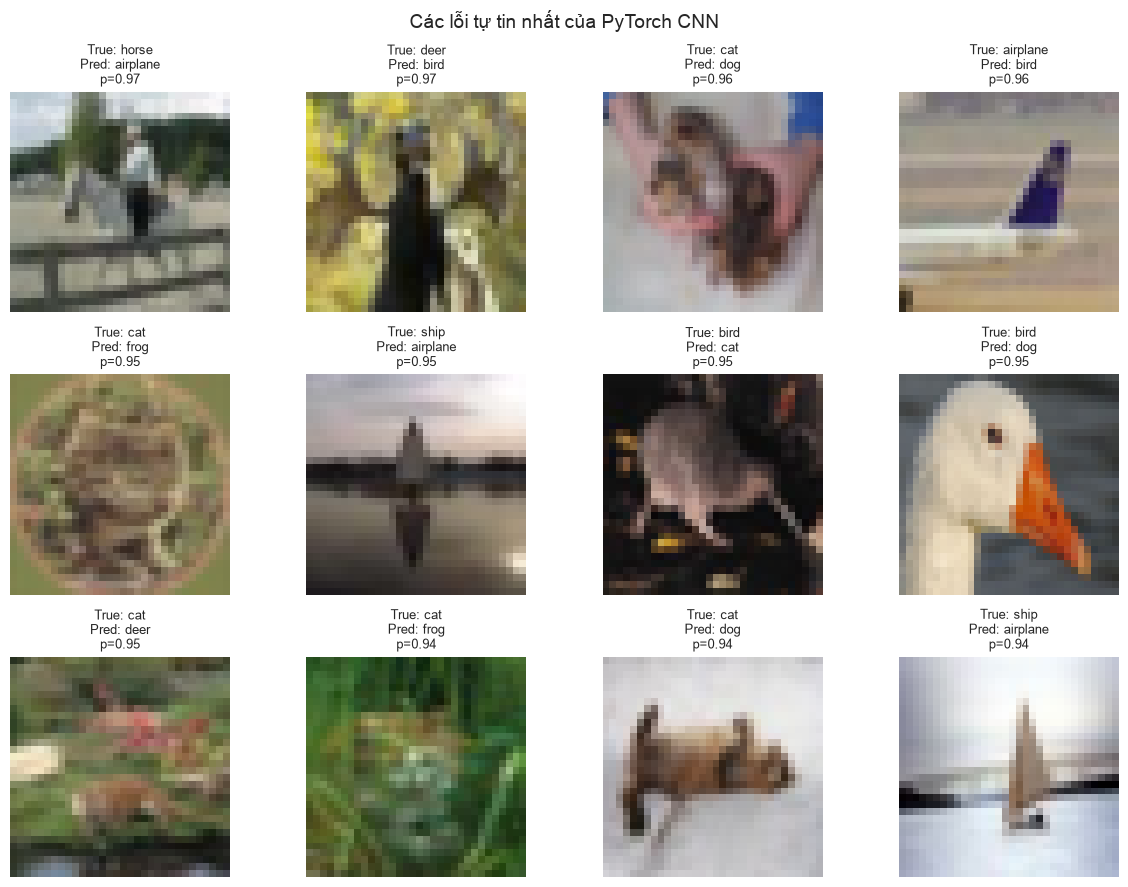
\includegraphics[width=0.88\textwidth]{cifar10_prediction_error_analysis.png}
    \caption{Các lỗi có confidence cao nhất của PyTorch CNN trên CIFAR-10}
    \label{fig:cifar_errors}
\end{figure}

Nhiều lỗi có tính mơ hồ ở độ phân giải $32\times32$: ngựa bị che khuất có thể
giống máy bay, hươu trong nền rừng giống chim, mèo/chó/chim bị nhầm do texture,
hoặc thuyền và máy bay cùng xuất hiện trên nền trời/nước. Trong ứng dụng thực tế,
có thể bổ sung calibration, dự đoán top-$k$ hoặc cơ chế từ chối khi confidence
không đáng tin cậy.

% =========================================================================
% CHUONG 5
% =========================================================================
\chapter{Đối chiếu tổng hợp và kết luận}

\section{Kết quả chính giữa hai dataset}
\begin{table}[H]
\centering
\caption{Mô hình tốt nhất và CNN NumPy trên mỗi dataset}
\label{tab:master_summary}
\resizebox{\textwidth}{!}{%
\begin{tabular}{lllllll}
\toprule
\textbf{Dataset} & \textbf{Mô hình} & \textbf{Accuracy} & \textbf{Macro-F1} & \textbf{Tham số} & \textbf{Train(s)} & \textbf{Dữ liệu train} \\
\midrule
MNIST & PyTorch CNN & 0.9958 & 0.9958 & 468,010 & 90.38 & 54,000 \\
MNIST & NumPy CNN & 0.9848 & 0.9847 & 52,138 & 82.86 & 20,000 \\
CIFAR-10 & PyTorch ResNet-20 & 0.9095 & 0.9092 & 272,474 & 822.82 & 45,000 \\
CIFAR-10 & NumPy CNN & 0.7012 & 0.6994 & 200,978 & 501.36 & 15,000 \\
\bottomrule
\end{tabular}%
}
\end{table}

Trên MNIST, CNN nông đã đủ mạnh: phiên bản NumPy chỉ kém mô hình tốt nhất khoảng
1.1 điểm phần trăm accuracy. Trên CIFAR-10, cùng thiết kế nông dừng ở khoảng
70\%, trong khi ResNet-20 vượt 90\%. So sánh này minh họa rằng độ phức tạp kiến
trúc cần phù hợp với độ phức tạp của dữ liệu.

\section{Vai trò của ba cách cài đặt}
\begin{table}[H]
\centering
\caption{Ưu điểm, hạn chế và vai trò của ba cách cài đặt}
\label{tab:implementation_tradeoff}
\small
\begin{tabularx}{\textwidth}{
    >{\raggedright\arraybackslash}p{3.0cm}
    >{\raggedright\arraybackslash}X
    >{\raggedright\arraybackslash}X
    >{\raggedright\arraybackslash}X}
\toprule
\textbf{Cách cài đặt} & \textbf{Ưu điểm} & \textbf{Hạn chế} & \textbf{Vai trò trong Assignment 04} \\
\midrule
NumPy from scratch & Minh bạch forward/backward, ít phụ thuộc & Chậm, khó mở rộng, dễ sai gradient & Hiểu thuật toán ở mức tensor \\
TensorFlow/Keras & API gọn, callback và pipeline dữ liệu tốt & Training loop ít tường minh hơn & Xây dựng baseline framework nhanh \\
PyTorch & Module và loop linh hoạt, debug thuận tiện & Phải tự quản lý nhiều trạng thái & Benchmark hiệu quả và kiểm soát rõ \\
\bottomrule
\end{tabularx}
\end{table}

CNN NumPy không nhằm thay thế framework trong triển khai quy mô lớn. Giá trị
chính của nó là làm rõ cache, mask pooling, sliding window, gradient và cập nhật
Adam. Keras và PyTorch phù hợp hơn khi cần residual blocks, tăng tốc phần cứng,
mixed precision hoặc mở rộng sang dữ liệu lớn.

\section{Giới hạn của phép đối chuẩn}
Các mô hình dùng cùng validation/test set và cùng metric trong từng dataset,
nhưng điều kiện huấn luyện không hoàn toàn giống nhau:
\begin{enumerate}
    \item NumPy dùng ít mẫu train hơn để giới hạn thời gian chạy;
    \item kiến trúc NumPy nông hơn, còn framework dùng ResNet-20 trên CIFAR-10;
    \item Keras \texttt{count\_params()} gồm cả trạng thái Batch Normalization
    không trainable, trong khi phép đếm PyTorch cộng các parameter của mô hình;
    \item thời gian phụ thuộc MPS, backend, graph compilation, warm-up và tải
    hệ thống tại thời điểm chạy;
    \item báo cáo chỉ có một random seed, chưa có trung bình và độ lệch chuẩn
    qua nhiều lần lặp.
\end{enumerate}
Vì vậy bảng kết quả trả lời câu hỏi ``pipeline nào hiệu quả trong đúng cấu hình
notebook này'' hơn là chứng minh framework nào luôn nhanh hoặc chính xác hơn.

\section{Khả năng tái lập}
\begin{table}[H]
\centering
\caption{Checklist tái lập Assignment 04}
\label{tab:reproducibility}
\resizebox{\textwidth}{!}{%
\begin{tabular}{lll}
\toprule
\textbf{Hạng mục} & \textbf{Cách thực hiện trong code} & \textbf{Ý nghĩa} \\
\midrule
Random seed & \texttt{RANDOM\_STATE = 42} cho NumPy/Keras/Torch & Giảm dao động split và khởi tạo \\
Tách dữ liệu & Stratified train/validation, test độc lập & Không chọn mô hình trên test \\
Chuẩn hóa & Mean/std chỉ học từ framework train & Chống data leakage \\
Checkpoint & NumPy theo val loss, framework theo val accuracy & Khôi phục trạng thái tốt nhất \\
Augmentation & Chỉ áp dụng cho mini-batch train & Giữ validation/test nguyên bản \\
Metric & Accuracy và macro P/R/F1 trên cùng test set & So sánh đa chiều \\
Hình ảnh & Xuất từ output notebook vào thư mục báo cáo & Truy vết được bảng và đồ thị \\
\bottomrule
\end{tabular}%
}
\end{table}

Output đã lưu ghi nhận NumPy 2.5.2, TensorFlow 2.21.0 và PyTorch 2.14.0; thiết
bị PyTorch là MPS. Để chạy lại đúng cấu trúc hiện tại:
\begin{enumerate}
    \item mở notebook trong \modelpath{Assignment4/<dataset>/notebook};
    \item bảo đảm thư mục \modelpath{../data} tồn tại để loader tải hoặc đọc dữ
    liệu cục bộ;
    \item chạy toàn bộ cell theo thứ tự từ cấu hình, load/split/normalize đến
    NumPy, Keras, PyTorch, benchmark và error analysis;
    \item xuất các đồ thị cần dùng vào
    \modelpath{Assignment4/Report/images/generated};
    \item biên dịch \modelpath{A04\_CT\_ThangDT.752.tex} bằng XeLaTeX hai lần để
    cập nhật mục lục và tham chiếu chéo.
\end{enumerate}

\section{Kết luận và hướng mở rộng}
Assignment 04 đã hiện thực và đối chuẩn ba cách xây dựng CNN trên MNIST và
CIFAR-10. CNN thuần NumPy bao gồm forward, backward, Adam, weight decay,
gradient clipping, cosine learning rate và augmentation. Trên MNIST, PyTorch
đạt Accuracy/Macro-F1 0.9958, Keras đạt 0.9955, còn NumPy đạt Accuracy 0.9848
và Macro-F1 0.9847. Trên CIFAR-10, PyTorch ResNet-20 đạt Accuracy 0.9095 và
Macro-F1 0.9092; Keras gần tương đương, trong khi CNN NumPy nông đạt Macro-F1
0.6994.

Kết quả cho thấy residual connection, Batch Normalization, augmentation, label
smoothing và lịch learning rate dài đặc biệt quan trọng đối với ảnh tự nhiên.
Phân tích lỗi cũng cho thấy các lớp gần nhau về hình dạng hoặc texture vẫn dễ bị
nhầm, rõ nhất là \textit{cat} và \textit{dog} trên CIFAR-10.

Hướng mở rộng gồm chạy nhiều seed để báo cáo độ ổn định, kiểm tra calibration,
thử mixup/cutout, dùng transfer learning và đo thêm throughput, bộ nhớ cùng kích
thước checkpoint. Với CNN NumPy, có thể tiếp tục vector hóa convolution hoặc sử
dụng Numba/CuPy để tách ảnh hưởng của thuật toán khỏi overhead vòng lặp Python.

\end{document}
